\documentclass[12pt,a4paper,oneside]{article}
\usepackage{olymp}
\usepackage{graphicx}
\usepackage{amsmath}
\usepackage{amssymb}
\usepackage{color} % for colored text
\usepackage{import} % for changing current dir
\usepackage{epigraph}
\usepackage{wrapfig} % for having text alongside pictures
\usepackage{verbatim}
\usepackage{ctex}
\usepackage{indentfirst}
\usepackage[table,xcdraw]{xcolor}
\setlength{\parindent}{2em}
% 子题目不再维护.

\begin{document}
\contest
{2023 Harbin Institute of Technology (Weihai) Newbie Programming Contest}%
{China, Shandong, Weihai}%
{December, 23, 2023}%

% ---------------------------------------------------------------------------------------------------------

    \begin{problem}{Personality Correction}{standard input}{standard output}{1 second}{256 megabytes}
	
    \textit{美国的凯恩琳·布里格斯和她的女儿伊莎贝尔·布里格斯·迈尔斯研制了迈尔斯-布里格斯类型指标(\textbf{MBTI})。这个指标以瑞士心理学家卡尔·荣格对人格划分的8种类型为基础,加以扩展,形成四个维度,即:}
    
    \begin{table}[htb]
        \centering
        \resizebox{\textwidth}{!}{%
        \begin{tabular}{|
        >{\columncolor[HTML]{FFFFFF}}c |
        >{\columncolor[HTML]{FFFFFF}}c |
        >{\columncolor[HTML]{FFFFFF}}c |
        >{\columncolor[HTML]{FFFFFF}}c |
        >{\columncolor[HTML]{FFFFFF}}c |}
        \hline
        {\color[HTML]{333333} \textbf{维度}}    & {\color[HTML]{333333} \textbf{类型}} & {\color[HTML]{333333} \textbf{相对应英文及缩写}} & {\color[HTML]{333333} \textbf{类型}} & {\color[HTML]{333333} \textbf{相对应英文及缩写}} \\ \hline
        {\color[HTML]{333333} 注意力方向(精力来源)}    & {\color[HTML]{333333} 外倾}          & {\color[HTML]{333333} E(Extrovert)}        & {\color[HTML]{333333} 内倾}          & {\color[HTML]{333333} I(Introvert)}       \\ \hline
        {\color[HTML]{333333} 认知方式(如何搜集信息)}   & {\color[HTML]{333333} 实感}          & {\color[HTML]{333333} S(Sensing)}          & {\color[HTML]{333333} 直觉}          & {\color[HTML]{333333} N(Intuition)}       \\ \hline
        {\color[HTML]{333333} 判断方式(如何做决定)}    & {\color[HTML]{333333} 思考}          & {\color[HTML]{333333} T(Thinking)}         & {\color[HTML]{333333} 情感}          & {\color[HTML]{333333} F(Feeling)}         \\ \hline
        {\color[HTML]{333333} 生活方式(如何应对外部世界)} & {\color[HTML]{333333} 判断}          & {\color[HTML]{333333} J(Judgment)}         & {\color[HTML]{333333} 感知}          & {\color[HTML]{333333} P(Perceiving)}      \\ \hline
        \end{tabular}%
        }
    \end{table}


    有一天,上帝注意到,这个世界的人格属性太不均匀了,于是想进行一次大人格修正。而你作为上帝的书记官,你的职责是帮助上帝完成修正工作。分配到你手上的是 $n$ 个人的人格属性分别为 $S_1, S_2, S_3, S_4 ... S_n$ ,上帝会对你下达两种指令:

        1. 给出一个 $l, r, c$ , $c \in \{E, I, S, N, T, F, J, P \}$, $c$ 为单一字符,表示将区间 $[l, r]$ 内的人的某维人格都修改为 $c$。
        
        2. 给出一个 $l, r, S$,  $S$ 为 \textbf{MBTI} 16人格中的某种人格, 例:ENFP 表示上帝想知道在区间 $[l,r]$ 内,有多少人是 ENFP 类型的;XNXP 表示上帝想知道在区间 $[l, r]$ 内,有多少人是 ENFP 或 ENTP 或 INFP 或 INTP 类型的。
	
	\InputFile
	第一行两个整数 $n (1 \leq n \leq 2 \times 10^3)$ ,$m (1 \leq      m \leq 2 \times 10^3)$ , 分别表示有 $n$ 个人和 $m$ 组询问。
        第二行包含 $n$ 个长度为 $4$ 的字符串 $S_i$,表示第 $i$ 个人的 \textbf{MBTI} 人格属性。
        接下来的 $m$ 行,表示 $m$ 个操作。具体如下:
        
            1.  $1 \ l \ r \ c$ : 表示将区间 $[l, r]$ 内的所有人的某维人格变为 $c$ 。
            
            2.  $2 \ l \ r \ S$ : 询问区间 $[l, r]$ 内人格属性为 S 的人的数量。
        \OutputFile
	输出若干整数,即所有操作 2 的结果。
	\Example
	
	\begin{example}
	\exmpfile{A/1.in}{A/1.ans}%
	\end{example}

    \Explanations
    一开始的人格序列为 INFP ENTP ENFJ INTJ ESTJ 。
    
    经过第一次修正之后,变成了 INFP ENTP ENTJ INTJ ESTJ 。
    
    之后查询区间 $[1,5]$ 之内所有的 INFP 发现只有第一个位置的人符合,答案为 1 。
    
    随后查询 XNTJ 即查询区间内 INTJ  和 ENTJ 的个数,分别为 3, 4 位置上两人,答案为2。
    
    随后将区间 $[1, 5]$ 内所有人格修正为 S  变成了 ISFP ESTP ESTJ ISTJ ESTJ。
    
    最后查询人格为 XSTP 的人,即查询 ISTP 和 ESTP 有几人,只有 2 位置的人符合,答案为 1。

    \textbf{tips}:
    没事的时候可以想想 $n = 10^5,m = 10^5$ 时怎么做。
	
\end{problem}
	
% ---------------------------------------------------------------------------------------------------------	

    \begin{problem}{Storm a City}{standard input}{standard output}{2 seconds}{256 megabytes}
	
        你是一个邪恶的巫师,正在攻击一座城市。
    
        在攻城过程中需要面对 $n$ 道城门,第 $i$ 城门的坐标可视为 $i$ , 强度为 $s_i $ 。你的任务是摧毁所有的城门,唯一的攻击手段——普通攻击效果如下:
        
        1. 攻击范围为 $k$ 。也就是说,可以攻击坐标为 $l, l + 1,... ,l + k - 1$ $(1 \le l \le l + k - 1 \le n)$ 的地方。 $(1 \le l \le l + k - 1 \le n)$ 。
        
        2. 初始攻击值为 $a$ 。
        
        3. 攻击范围位置 $l, l + 1,\dots ,l + k - 1$ ,所对应的攻击力为 $a, a + 1,\dots ,a + k - 1$ 。
        
        当 $i$ 号城门受到的攻击总数为 $T _i \ge s_i$ 时, $i$ 号城门会被摧毁。
        
        问:要攻破所有城门,最少需要多少次普通攻击?
        
	\InputFile

        第一行包含三个整数 $n, k$ 和 $a$ ,分别代表城门数量、法师攻击范围和初始攻击值 $a$ 。
        
        第二行包含 $n$ 个整数, $s_1, s_2,... , s_n$ 表示城门的强度。
        
        $1 \le k \le n \le 5\times 10^{5}$ 、 $1 \le a \le 10^{5}$ 、 $1 \le s_i \le 10^{16}$ 。
        \OutputFile
	输出一行一个整数,表示要执行的最少普通攻击次数。
	\Example
	
	\begin{example}
	\exmpfile{B/1.in}{B/1.ans}%
        \exmpfile{B/2.in}{B/2.ans}%
	\end{example}
	\Explanations
        在示例 1 中 :

        一个可能的方案是:对 $[1, 3]$ 进行 $3$ 次攻击,对 $[4, 6]$ 进行 $1$ 次攻击,对 $[5, 7]$ 进行 $1$ 次攻击。可以证明没有更少的攻击次数。
	
\end{problem}

% ---------------------------------------------------------------------------------------------------------	

    \begin{problem}{Campus Network}{standard input}{standard output}{1 second}{256 megabytes}
	
	\textit{星雨晨曦}想要入坑明日方舟,现在他需要下载它。
 
	已知明日方舟所占用的内存空间是 2 GB,校园网的网速是 $x$ KB/s($1 \le x \le 5000$,保证 $x$ 为整数),\textit{星雨晨曦}想知道经过多少秒他可以下载完成(向上取整)。
	
        已知:1GB=1024MB,1MB=1024KB。

	
	\InputFile
	一行一个整数$x(1 \le x \le 5000)$,表示校园网网速。
	
	\OutputFile
	一行一个整数 $t$,表示\textit{星雨晨曦}经过 $t$ 秒后可以下载完成,时间 $t$ 向上取整。
	
	\Example
		
	\begin{example}
	\exmpfile{C/1.in}{C/1.ans}%
        \exmpfile{C/2.in}{C/2.ans}%
        \exmpfile{C/3.in}{C/3.ans}%
	\end{example}
	
	\end{problem}

 % ---------------------------------------------------------------------------------------------------------	
    
    \begin{problem}{Prime(Easy)}{standard input}{standard output}{1 second}{256 megabytes}
	
	

    2022年ICPC杭州站是英文题面。
    
    2023年ICPC杭州站增加了中文题面。
    
    于是这道题再次精简,变成一句话题意。

    

    给定一个整数 $n \ (1 \leq n \leq 10^4)$ ,你需要求出 $1 \sim n$ 中回文质数的数量。

	
	
	\InputFile
	
	一个整数 $T\ (1\leq T \leq 5)$,表示输入的数据组数。
        对于每组数据,输入一个整数 $n \ (1 \leq n \leq 10^4)$ 。

	
	\OutputFile
	
	一行一个整数,表示 $1 \sim n$ 中回文质数的数量。
	
	\Example
 
	\begin{example}
	\exmpfile{D/1.in}{D/1.ans}%
	\end{example}
	\Note
    数据范围:$1\leq T \leq 5$, $1 \leq n \leq 10^4$。
    
    回文数:如果一个数正着读和倒着读都一样的话,那么这个数就是回文数,如“7”,“12321”,“5665”。
	\end{problem}


	% ---------------------------------------------------------------------------------------------------------	
	
	\begin{problem}{Prime(Hard)}{standard input}{standard output}{2.5 seconds}{256 megabytes}

        ------------
        
        \textit{给予我生命的…是您}
        
        \textit{我一直爱着您…}
        
        \textit{虽然给您添了很多麻烦…我还是非常感谢能和您在这个世界再次相遇…}
        
    	\textit{在只能一个人前进的路上,还赐予了我这段美好的时间…}
    	
        \textit{在被你称作幻想世界的这个世界中的生活,对我来说是至高无上的美好回忆}
    	
        \textit{这个梦之世界,才是我人生中最重要的记忆…}
        
        \textit{终于,在这趟列车的重点,高岛同学的身体化为点点星光,消散在这璀璨的星河中。}
        
        \textit{我伸出手,想要抓住她的残影——}
        
        \textit{但视线中却是坐在床边满脸担忧的若{\CJKfontspec{simsun.ttc} 槻}司和侧过脸的若{\CJKfontspec{simsun.ttc} 槻}镜。}
        
        \textit{“你还好吗,有哪里不舒服吗,由岐?”作为妹妹的司攥着我的手关切地问道。}
        
        \textit{紧接着镜也用着别扭的音调回了一句:“又是做什么噩梦了吧,大概也没什么……大概。”}
        
        \textit{“柘榴同学呢?”}
        
        \textit{在我突然的发言后,她们的神情变得奇怪起来,像是不明白我为什么会说出这个名字一般。}
        
        \textit{“柘榴同学她……”}
        
        \textit{“从那么高的楼上掉下来,昨天还闹出了好大的动静来着,唉,怎么会这样,她平时……”}
        
        \textit{其他的声音都已经传达不到耳中,我只是在反复重复着这两个词:“高楼”和“坠落”。}

        ------------
        
        \textit{水上由岐}记得,那位在楼顶往下扔着玩偶的奇怪少女,在第一次见面的时候,不仅和她说了夏季大三角,还有\textbf{她喜欢的数字}。
        
        “727,是个很神奇的数字吧,※ \textbf{正着念和倒着念都是一样}的呢。”
        
        “还有,它 ※ \textbf{不会被任何小于它的数整除哦,除了1以外}。”
        
        “想和由岐去看夏季大三角,一起听做梦的鱼,一起去往7月27号呢。”说到这里,少女站上护栏边沿,看着被夕阳逐渐染红的天空,“不过,这个世界会在7月20号迎来终结吧……”
        
        记忆就此终断,水上由岐想知道\textbf{柘榴喜欢的数字}在给定界限内有多少个。


        给定范围 $n\ (1 \le n \le  10^9)$,由岐想要知道 $1 \sim n$ 中\textbf{柘榴喜欢的数字}有多少(假定所有满足上述两个条件的数都为柘榴喜欢的数)


		
		\InputFile
		
		
        一个整数 $T\ (1\leq T \leq 10000)$ 表示输入数据的组数。
        
        接下来 $T$ 行每行输入一个数字 $n \ (1 \leq n \leq   10^9)$ 表示给定的界限。
		\OutputFile
		每行输出一个整数,表示对应范围 $1 \sim n$ 内柘榴喜欢的数的数量。
		
		\Example
		
		\begin{example}
			\exmpfile{E/1.in}{E/1.ans}%
		\end{example}

        \Note
        
        数据范围: $1\leq T \leq 10000$, $1 \leq n \leq  10^9$。
        
        注意:\textbf{一位数正着念和倒着念也一样},1\textbf{不是}柘榴喜欢的数字
	\end{problem}
	


% ---------------------------------------------------------------------------------------------------------	

    \begin{problem}{Hurry,Hurry,Hurry!Route to Building M!}{standard input}{standard output}{2 seconds}{256 megabytes}
	
        \textit{Kersen 是哈尔滨工业大学(威海)的一名大一新生。某天早上 7:50,8:00 有课但仍在寝室睡大觉的 Kersen 刚刚从梦中醒来。现在是时候赶往 M 楼了!}
        
        哈尔滨工业大学(威海)有 $n$ 条道路,这 $n$ 条道路可以在任意位置相互交叉,并且\textbf{不存在单行线}。正赶往 M 楼的 \textit{Kersen} 只能走给定的道路,且可以通过道路之间的交叉点从一条道路移动到另一条道路。为了简化模型,我们将学校看作一个\textbf{二维的平面},每条道路可以看作\textbf{一条线段}, \textit{Kersen} 的寝室和 M 楼都可以看作两个点。保证寝室和 M 楼一定在道路上(但不保证一定为道路的端点),并且在所有线段中任选的两个点一定能相互到达(即图是联通的)。
        
        由于对学校还不够熟悉,\textit{Kersen} 并不知道从寝室到 M 楼需要多远。好消息是,由于学校的数字化系统非常完善,他能够得知所有楼和道路端点在平面直角坐标系下的坐标。他想知道自己是否还有足够的时间赶往 M 楼。他非常着急!他已经没有时间思考了!现在,请你告诉他问题的答案!
	
	\InputFile
	
	输入共有 $n+2$ 行。
        
        第一行包含一个正整数 $n$ $(1 \leq n \leq 100)$,表示道路的数量。
        
        第二行包含四个整数 $x_s, y_s, x_m, y_m (-10000 \leq x_s, y_s,x_m,y_m \leq 10000)$ 分别表示 Kersen 的寝室和 M 楼的坐标。 
        
        第 $3$ 行到第 $n+2$ 行,每行包含四个整数 $x_1, y_1, x_2, y_2 (-10000 \leq x_1, y_1,x_2,y_2 \leq 10000)$ ,表示每条道路的两个端点坐标。  
	
	\OutputFile
	
	输出一行一个实数,表示从 \textit{Kersen} 寝室到 M 楼的最短距离。

        当你的答案被认为是正确的当且仅当它与标准答案之间的绝对误差或相对误差小于 $10^{-6}$ 。

        更准确的来说,假设你的答案是 $x$ 、标准答案为 $y$,那么你的答案将被认为是正确的当且仅当 $\frac{|x-y|}{max(1,|y|)} < 10^{-6}$ 。
	
	\Example
	
	\begin{example}
	\exmpfile{F/1.in}{F/1.ans}%
	\end{example}
	
	\Explanations
    \begin{center}
	  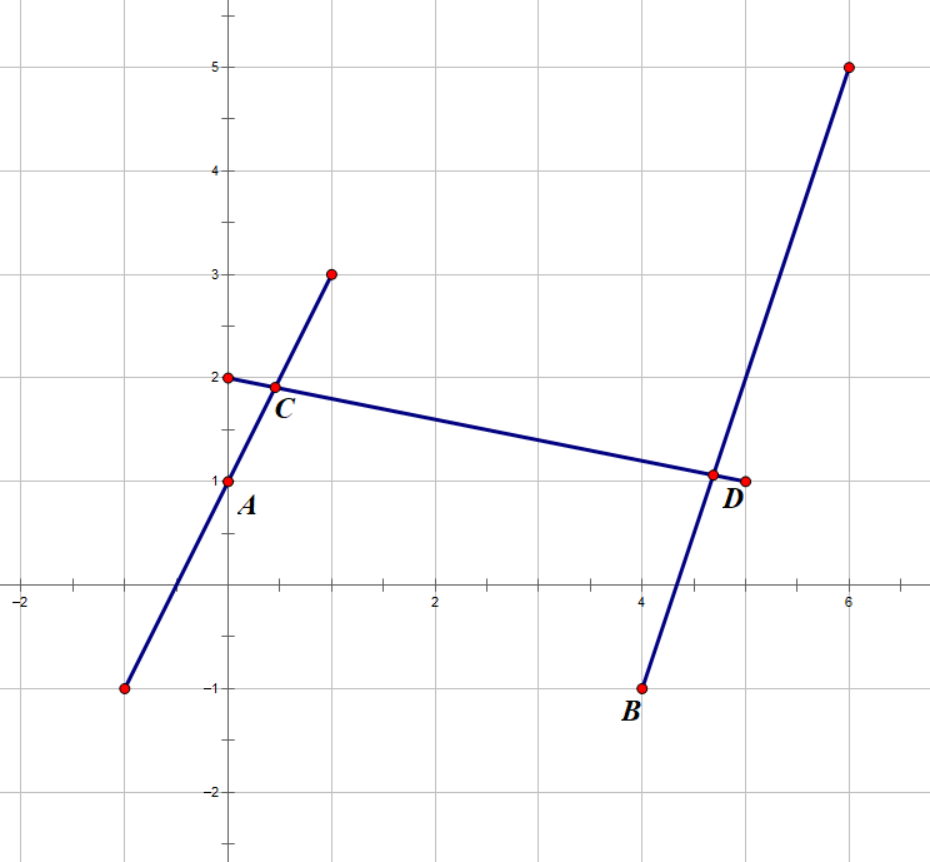
\includegraphics[width=0.7\linewidth]{F/testcase.png}
	\end{center}
    如上图所示,在该样例中,\textit{Kersen} 的寝室在 $A$ 点,M楼在 $B$ 点。  
    \textit{Kersen}从寝室到M楼的最短路径为 $A\rightarrow C \rightarrow D \rightarrow B$,该路径的长度为7.5072439921。
	
	\end{problem}

% ---------------------------------------------------------------------------------------------------------	

    \begin{problem}{Gacha}{standard input}{standard output}{1 second}{256 megabytes}
	
	在游戏《明日方舟》中,玩家有如下方式获得\textbf{抽卡}资源:
 
        1.每周一刷新的剿灭作战任务,完成可以获得1800\textbf{合成玉}。
        
        2.每周二游戏会自动进行闪断更新,系统自动发放200\textbf{合成玉}。
        
        3.每周刷新的周常任务,完成可以获得500\textbf{合成玉}。
        
        4.每天刷新的日常任务,完成可以获得100\textbf{合成玉}。

        5.如果购买了月卡,可以立即获得6\textbf{源石}并将月卡的持续时间加30天,月卡生效的时间内每天可以获得200\textbf{合成玉}。
        
        6.大月卡一次性获得42\textbf{源石}以及 10 次\textbf{抽卡}机会(十抽)。

        每颗\textbf{源石}可以换取180\textbf{合成玉},每600\textbf{合成玉}可以获得 1 次\textbf{抽卡}机会。

        \textit{星雨晨曦}是一名勤奋的明日方舟玩家,他每天都会登陆明日方舟完成日常任务,并且每周一完成剿灭作战任务,每周三完成周常任务。假设今天是第一天且为周一,他想知道自己在第 $x$ 天结束后会积累多少次\textbf{抽卡}机会。

        \textit{星雨晨曦}会在这 $x \ (1 \le x \le 1000)$ 天内氪金若干次\textbf{月卡}或\textbf{大月卡}。

	\InputFile
	第一行三个整数 $x,n,m$,$x$ 表示\textit{星雨晨曦}想知道他在第 $x$ 天结束后会积累多少次抽卡机会,$n$ 表示他会氪金 $n$ 次月卡,$m$ 表示他会氪金 $m$ 次大月卡。
 
        第二行输入 $n$ 个数 $a_1,a_2,a_3,\dots ,a_n$,$a_i$ 表示\textit{星雨晨曦}购买\textbf{月卡}所在天数。

        第三行输入 $m$ 个数 $b_1,b_2,b_3,\dots ,b_m$,$b_i$ 表示\textit{星雨晨曦}购买\textbf{大月卡}所在天数。

        数据范围为 $1 \le x,a_i,b_i \le 1000$,$0 \le n,m \le 30$ 。
        
        且 $a_i,b_i$ 满足 $a_1 < a_2 < a_3 < \dots < a_n$, $b_1 < b_2 < b_3 < \dots < b_m$。
	
	\OutputFile
	
	输出一行一个整数 ,表示\textit{星雨晨曦}在第 $x$ 天结束后会积累多少次抽卡机会。

	
	\Example
	
	\begin{example}
	\exmpfile{G/1.in}{G/1.ans}%
	\exmpfile{G/2.in}{G/2.ans}%
	\end{example}
    \Explanations
    对于样例1,\textit{星雨晨曦} 在第 1 天完成了剿灭作战任务,获得了1800 合成玉;第2天游戏进行闪断更新,系统自动发放 200 合成玉;第3天完成周常任务,获得500合成玉。
    
    除此以外,他每天完成日常任务,3天共获得300合成玉。
    
    第2天他氪金了月卡,他当即获得 6 源石即 1080 合成玉,并在$2 \sim 3$ 天内每天获得200合成玉共400合成玉。

    第3天他氪金了大月卡,当即获得42源石即7560合成玉,并额外获得10次抽卡机会。


    至此他有 $1800+200+500+300+1080+400+7560=11840$ 合成玉,可以获得$\lfloor \frac{11840}{600} \rfloor = 19$ 次抽卡机会,合计获得29次抽卡机会。
    \Note
    注意:每周二游戏会自动进行闪断更新,系统自动发放200\textbf{合成玉}。

    \textbf{月卡}不仅当即有\textbf{源石}发放,也有持续时间的概念。而\textbf{大月卡}所有奖励一次性发放。
    \end{problem}

% ---------------------------------------------------------------------------------------------------------	
	\begin{problem}{Ball}{standard input}{standard output}{1 second}{256 megabytes}
		
	\textit{Asdfo} 最近迷上了摸球。

        \textit{Asdfo} 不喜欢重复,因此球有\textbf{颜色}和\textbf{编号}两种属性,只要有一个不同就视为不同的球。
        
        \textit{Asdfo} 不喜欢重复,因此他买了 $n + m$ 种颜色的球。其中前 $n$ 种颜色的球各有 $a$ 个,编号为 $1$ 到 $a$。后 $m$ 种颜色的球各有 $b$ 个,编号为 $1$ 到 $b$。$(0 \le n, m, a, b \le 10^3 )$ 
        
        \textit{Asdfo} 不喜欢重复,因此他每次会从中摸出 $k$ 个颜色互不相同的球。
        
        \textit{Asdfo} 不喜欢重复,因此他希望被摸出来的球的编号互不相同。
        
        当然,\textit{Asdfo} 学过生日悖论,他知道当 $k$ 足够大时,这个概率是很低的。但 \textit{Asdfo} 还是不喜欢重复,因此他希望知道,存在多少个\textbf{大小}为 $k$ 且\textbf{颜色、编号互不相同}的球的集合。

        这个数字可能很大,你只需要输出答案 $mod \ \ 998, 244, 353 $ 的结果即可。
	
	\InputFile
	从标准输入读入数据。

        第一行包含 $5$ 个正整数 $n, m, a, b, k$,含义如题面所示。$(0 \le n, m, a, b \le 10^3, \ 0 \le k \le n + m)$
	
	\OutputFile
	输出到标准输出。输出一个非负整数,表示满足条件的集合个数 $mod \ \ 998, 244, 353$ 的结果。
	
	\Example
	\begin{example}
	\exmpfile{H/1.in}{H/1.ans}%
	\end{example}
        \Explanations
        假设球 $(x, y)$ 表示颜色为 $x$ ,编号为 $y$  的球。

        大小为 $2$,颜色互不相同、编号互不相同的球的集合有 $\{{(1, 1),(2, 2)}\}$ , $\{{(1, 1),(3, 2)}\}$ , $\{{(2, 1),(3, 2)}\}$ , $\{{(2, 2), (3, 1)}\}$ , 一共 $4$ 个。
        
        \newpage
	\Note
        在 $xCPC$ 比赛中,有很多时候会遇到大数取模问题:

        比如,我们要求一个数的阶乘对某数取模的结果,或者斐波那契数列中后面的项对某个数取模的结果。如果不取模,这些数字用int 或者 long long 类型是存不下的。为了防止溢出,我们将这些数字取模,在运算中取模问题有以下几个公式:
        
            1. 两数相加再取模
               $(m + n) \% p = (m\%p + n\%p) \%p$
               
            2. 两数相乘再取模
               $(m * n) \% p = (m\%p * n\%p) \%p$
               
            3. 两数相减再取模
               $(m - n) \% p = (m\%p - n\%p + p) \%p$
               

        对于上面的公式,在三个数及以上的时候也可以使用,用法因具体情况而异。
	\end{problem}


% ---------------------------------------------------------------------------------------------------------	


\end{document}